\setbeamercolor{background canvas}{bg=fitblue}
\begin{frame}
\frametitle{Barva}
\begin{center}
\Huge {\color{white}Barva}
\end{center}
\end{frame}
\setbeamercolor{background canvas}{bg=white}


\begin{frame}
    \frametitle{Barva}
    \begin{columns}[c]
    \column{.5\textwidth}
        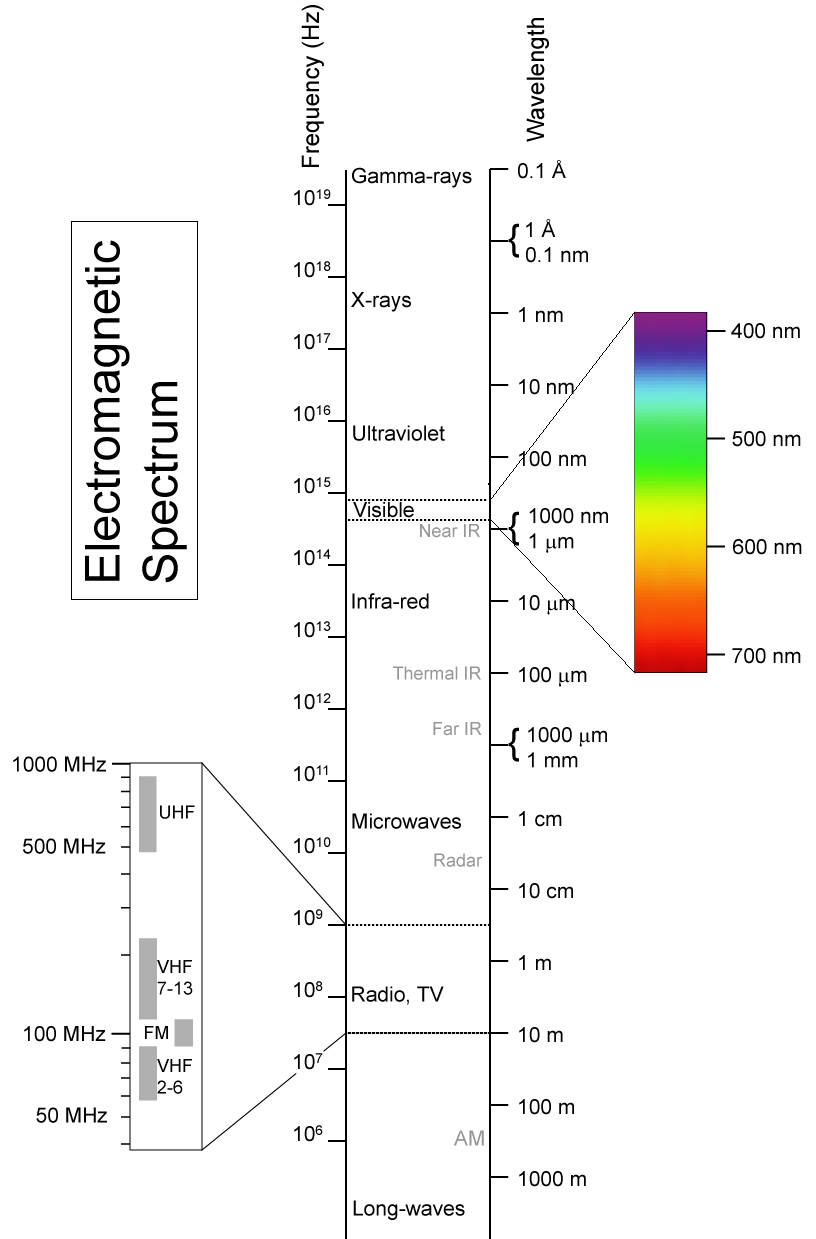
\includegraphics[height=\textheight]{pics/color/Electromagnetic-Spectrum.eps}
    \column{.5\textwidth}
        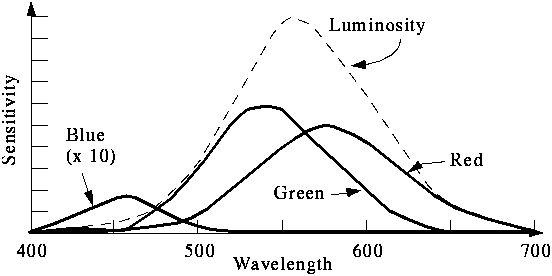
\includegraphics[width=\textwidth]{pics/color/citlivost-oka.eps}

        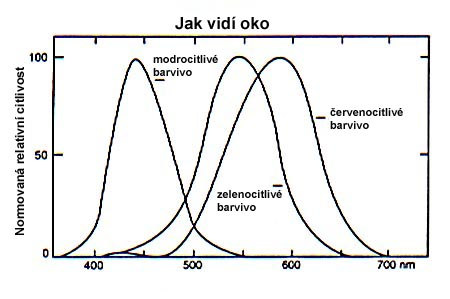
\includegraphics[width=\textwidth]{pics/color/citlivost-oka-normovana.eps}
    \end{columns}
\end{frame}

\begin{frame}
    \frametitle{Gamut}
    \begin{columns}[c]
    \column{.5\textwidth}
        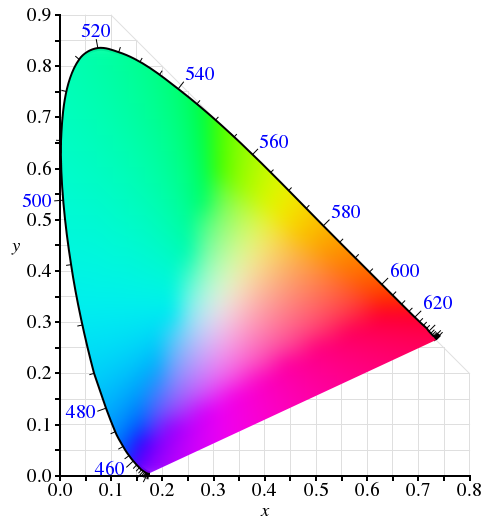
\includegraphics[width=\textwidth]{pics/color/gamut.eps}
    \column{.5\textwidth}
        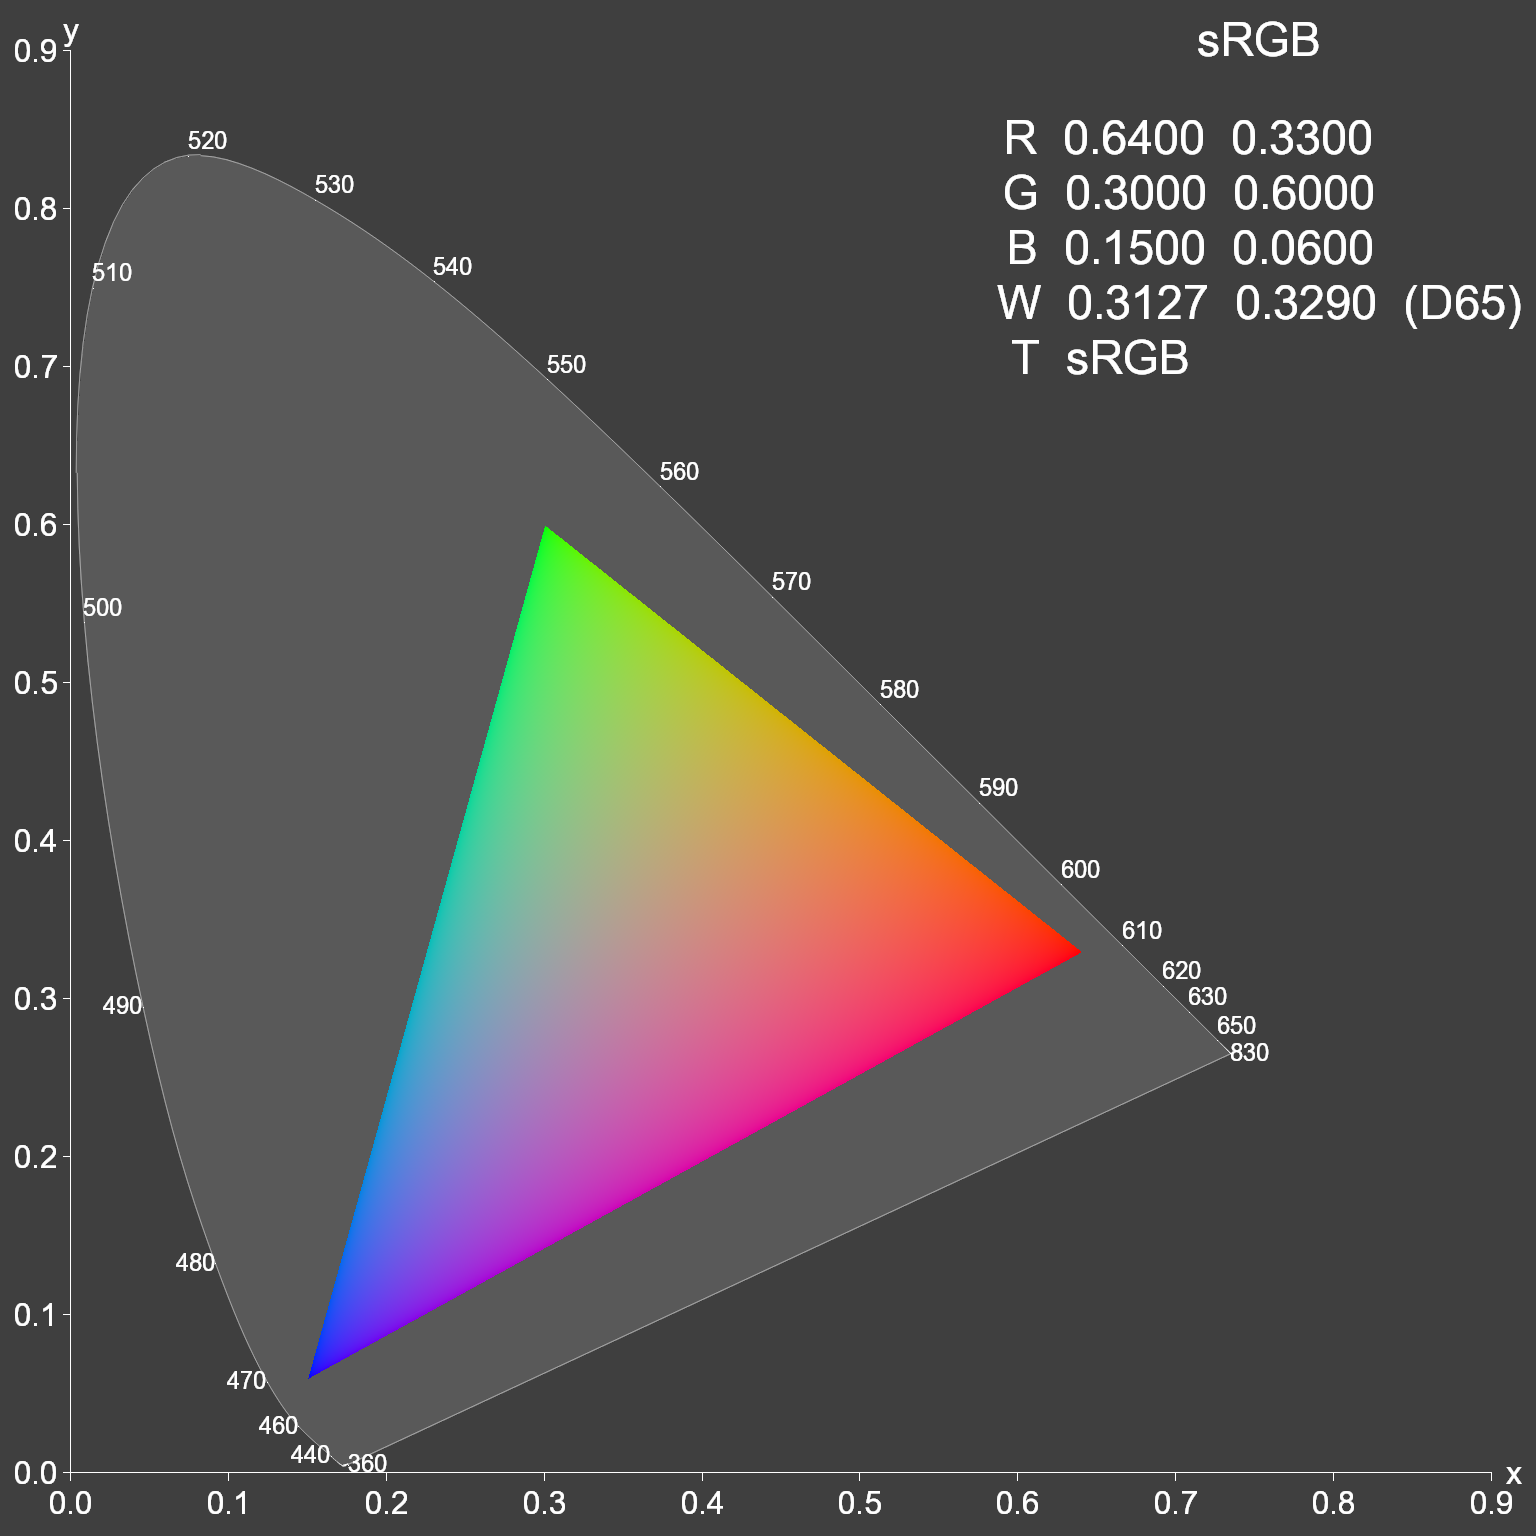
\includegraphics[width=\textwidth]{pics/color/Gamut-sRGB.eps}
    \end{columns}
    \vfill
    \begin{itemize}
        \item CIE 1931
        \item XYZ vs RGB
    \end{itemize}
\end{frame}

\begin{frame}
    \frametitle{Gamma}

    \begin{columns}[c]
    \column{.5\textwidth}
        Logaritmická citlivost oka

        \begin{eqnarray*}
        C_\mathrm{srgb}=\begin{cases}
        12.92C_\mathrm{l}, & C_\mathrm{l} \le t\\
        (1+a)C_\mathrm{l}^{\frac{1}{2.4}}-a, & C_\mathrm{l} > t
        \end{cases} \\
        a = 0.055 \\
        t = 0.0031308
        \end{eqnarray*}
        
    \column{.5\textwidth}
        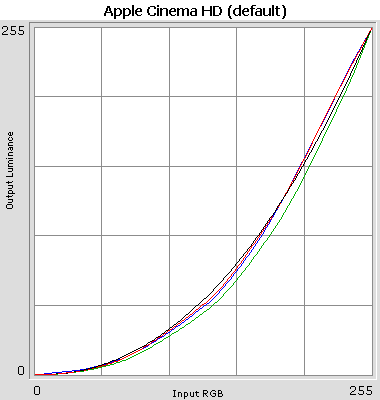
\includegraphics[width=\textwidth]{pics/color/monitor.eps}
    \end{columns}
\end{frame}

\begin{frame}
    \frametitle{Barva v OpenGL}

    Pipeline :
    \begin{itemize}
        \item float RGB(A) (vec3)
        \item {\color{black}$(0,0,0)$ \color{red}$(1,0,0)$ \color{green}$(0,1,0)$ \color{blue}$(0,0,1)$}
        \item[\color{red}!] Lineární barevný prostor - interpolace, blending.
    \end{itemize}
    \pause\vfill
    Vstupy a framebuffer :
    \begin{itemize}
        \item Nejčastější RGB8
        \item Další : RGB16, RGB565, ...
        \item Lineární, nebo sRGB
        \item Ruční konverze?
        \item glEnable(GL\_SRGB);
    \end{itemize}
\end{frame}

